\documentclass[a4paper]{article}

\usepackage{times}
\usepackage[ngerman]{babel}
\usepackage[T1]{fontenc}
\usepackage{amsmath}
\usepackage{amsfonts}
\usepackage{graphicx}
\usepackage{authblk}
\usepackage{fancyhdr}

\pagestyle{fancy}
\renewcommand{\headrulewidth}{0,6pt}
\fancyhead[L]{\leftmark}
\fancyhead[R]{\thepage}

\title{\Huge{Elektrik\\Lernzettel}}
\date{\today}
\author{\quad\\Baden, Julian\\Hagemann, Florian\\\quad\\Gymnasium Mellendorf\\ABI Jahr 2027}

\begin{document}

\maketitle
\thispagestyle{empty}
\newpage
\tableofcontents \thispagestyle{empty}
\newpage
\pagenumbering{arabic}

%________________________________________________________________________________________________

\section{Formelsammlung}
\subsection{Einheiten}

\begin{center}
    \begin{tabular}{ p{4cm} p{4cm} p{4cm} }
         Stromstärke            & $I$           & $A$                 \\[0,5cm]
         Ladung                 & $Q$ ($q$ für eine Probeladung)  & $C$ \\[0,5cm]
         Spannung               & $U$           & $V$                 \\[0,5cm]
         Wiederstand            & $R$           & $\Omega$            \\[0,5cm]
         el. Feldstärke         & $\vec{E}$     & $\dfrac{N}{C}$      \\[0,5cm]
         Kapazität              & $C$           & $F$                 \\[0,5cm]
         Flächenladungsdichte   & $\sigma$      & $\dfrac{C}{m^2}$    \\[1cm]
    \end{tabular}
\end{center}


\subsection{Formeln}
\paragraph{Stromstärke}
\large{$$I = \dfrac{Q}{t}$$}

\paragraph{Spannung}
\large{$$U = R \cdot I$$}




\section{Schaltungen}
\subsection{Schaltungen von Widerständen}

\paragraph{Reihe}

\begin{center}
	\Large
		$I_{ges} = I_1 = I_2 = … = I_n$\\[0,5cm]
		$U_{ges} = U_1 + U_2 + … + U_n$\\[0,5cm]
		$R_{ges} = R_1 + R_2 + … + R_n$\\[1cm]
	\normalsize
\end{center}


\paragraph{Parallel}

\begin{center}
	\Large
		$I_{ges} = I_1 + I_2 + … + I_n$\\[0,5cm]
		$U_{ges} = U_1 = U_2 = … = U_n$\\[0,5cm]
		$\dfrac{1}{R_{ges}} = \dfrac{1}{R_1} + \dfrac{1}{R_2} + … + \dfrac{1}{R_n}$\\[1cm]
	\normalsize
\end{center}


\paragraph{Kirchhoff‘schen Gesetze (Bei Knotenpunkten)}

\begin{center}
    \Large 
        $\sum{I_{zufließend}} = \sum{I_{abfließend}}$\\[1cm]
    \normalsize
\end{center}



\subsection{Schaltungen von Kondensatoren}

\paragraph{Reihe}

\begin{center}
	\Large
		$Q_{ges} = Q_1 + Q_2 + … + Q_n$\\[0,5cm]
		$U_{ges} = U_1 + U_2 + … + U_n$\\[0,5cm]
		$\dfrac{1}{C_{ges}} = \dfrac{1}{C_1} + \dfrac{1}{C_2} + … + \dfrac{1}{C_n}$\\[1cm]
	\normalsize
\end{center}


\paragraph{Parallel}

\begin{center}
	\Large
		$Q_{ges} = Q_1 + Q_2 + … + Q_n$\\[0,5cm]
		$U_{ges} = U_1 = U_2 = … = U_n$\\[0,5cm]
		$C_{ges} = C_1 + C_2 + … + C_n$\\[1cm]
	\normalsize
\end{center}


\section{Elektrische Felder}

\subsection{Radialsymetrische Felder}
Bei Radialsymetrischen Feldern treten die Feldlinien radial (also sekrecht)
aus einer positiven Punktladung hervor.

\begin{figure} [h]
	\begin{center}
		\includegraphics[width=8cm]{Bilder/feldlinien_punktladung.png}
		\caption{Feldlinien von Punktladungen}
	\end{center}
\end{figure}

Feldlinien führen immer von + zu -.

\begin{figure} [h]
	\begin{center}
		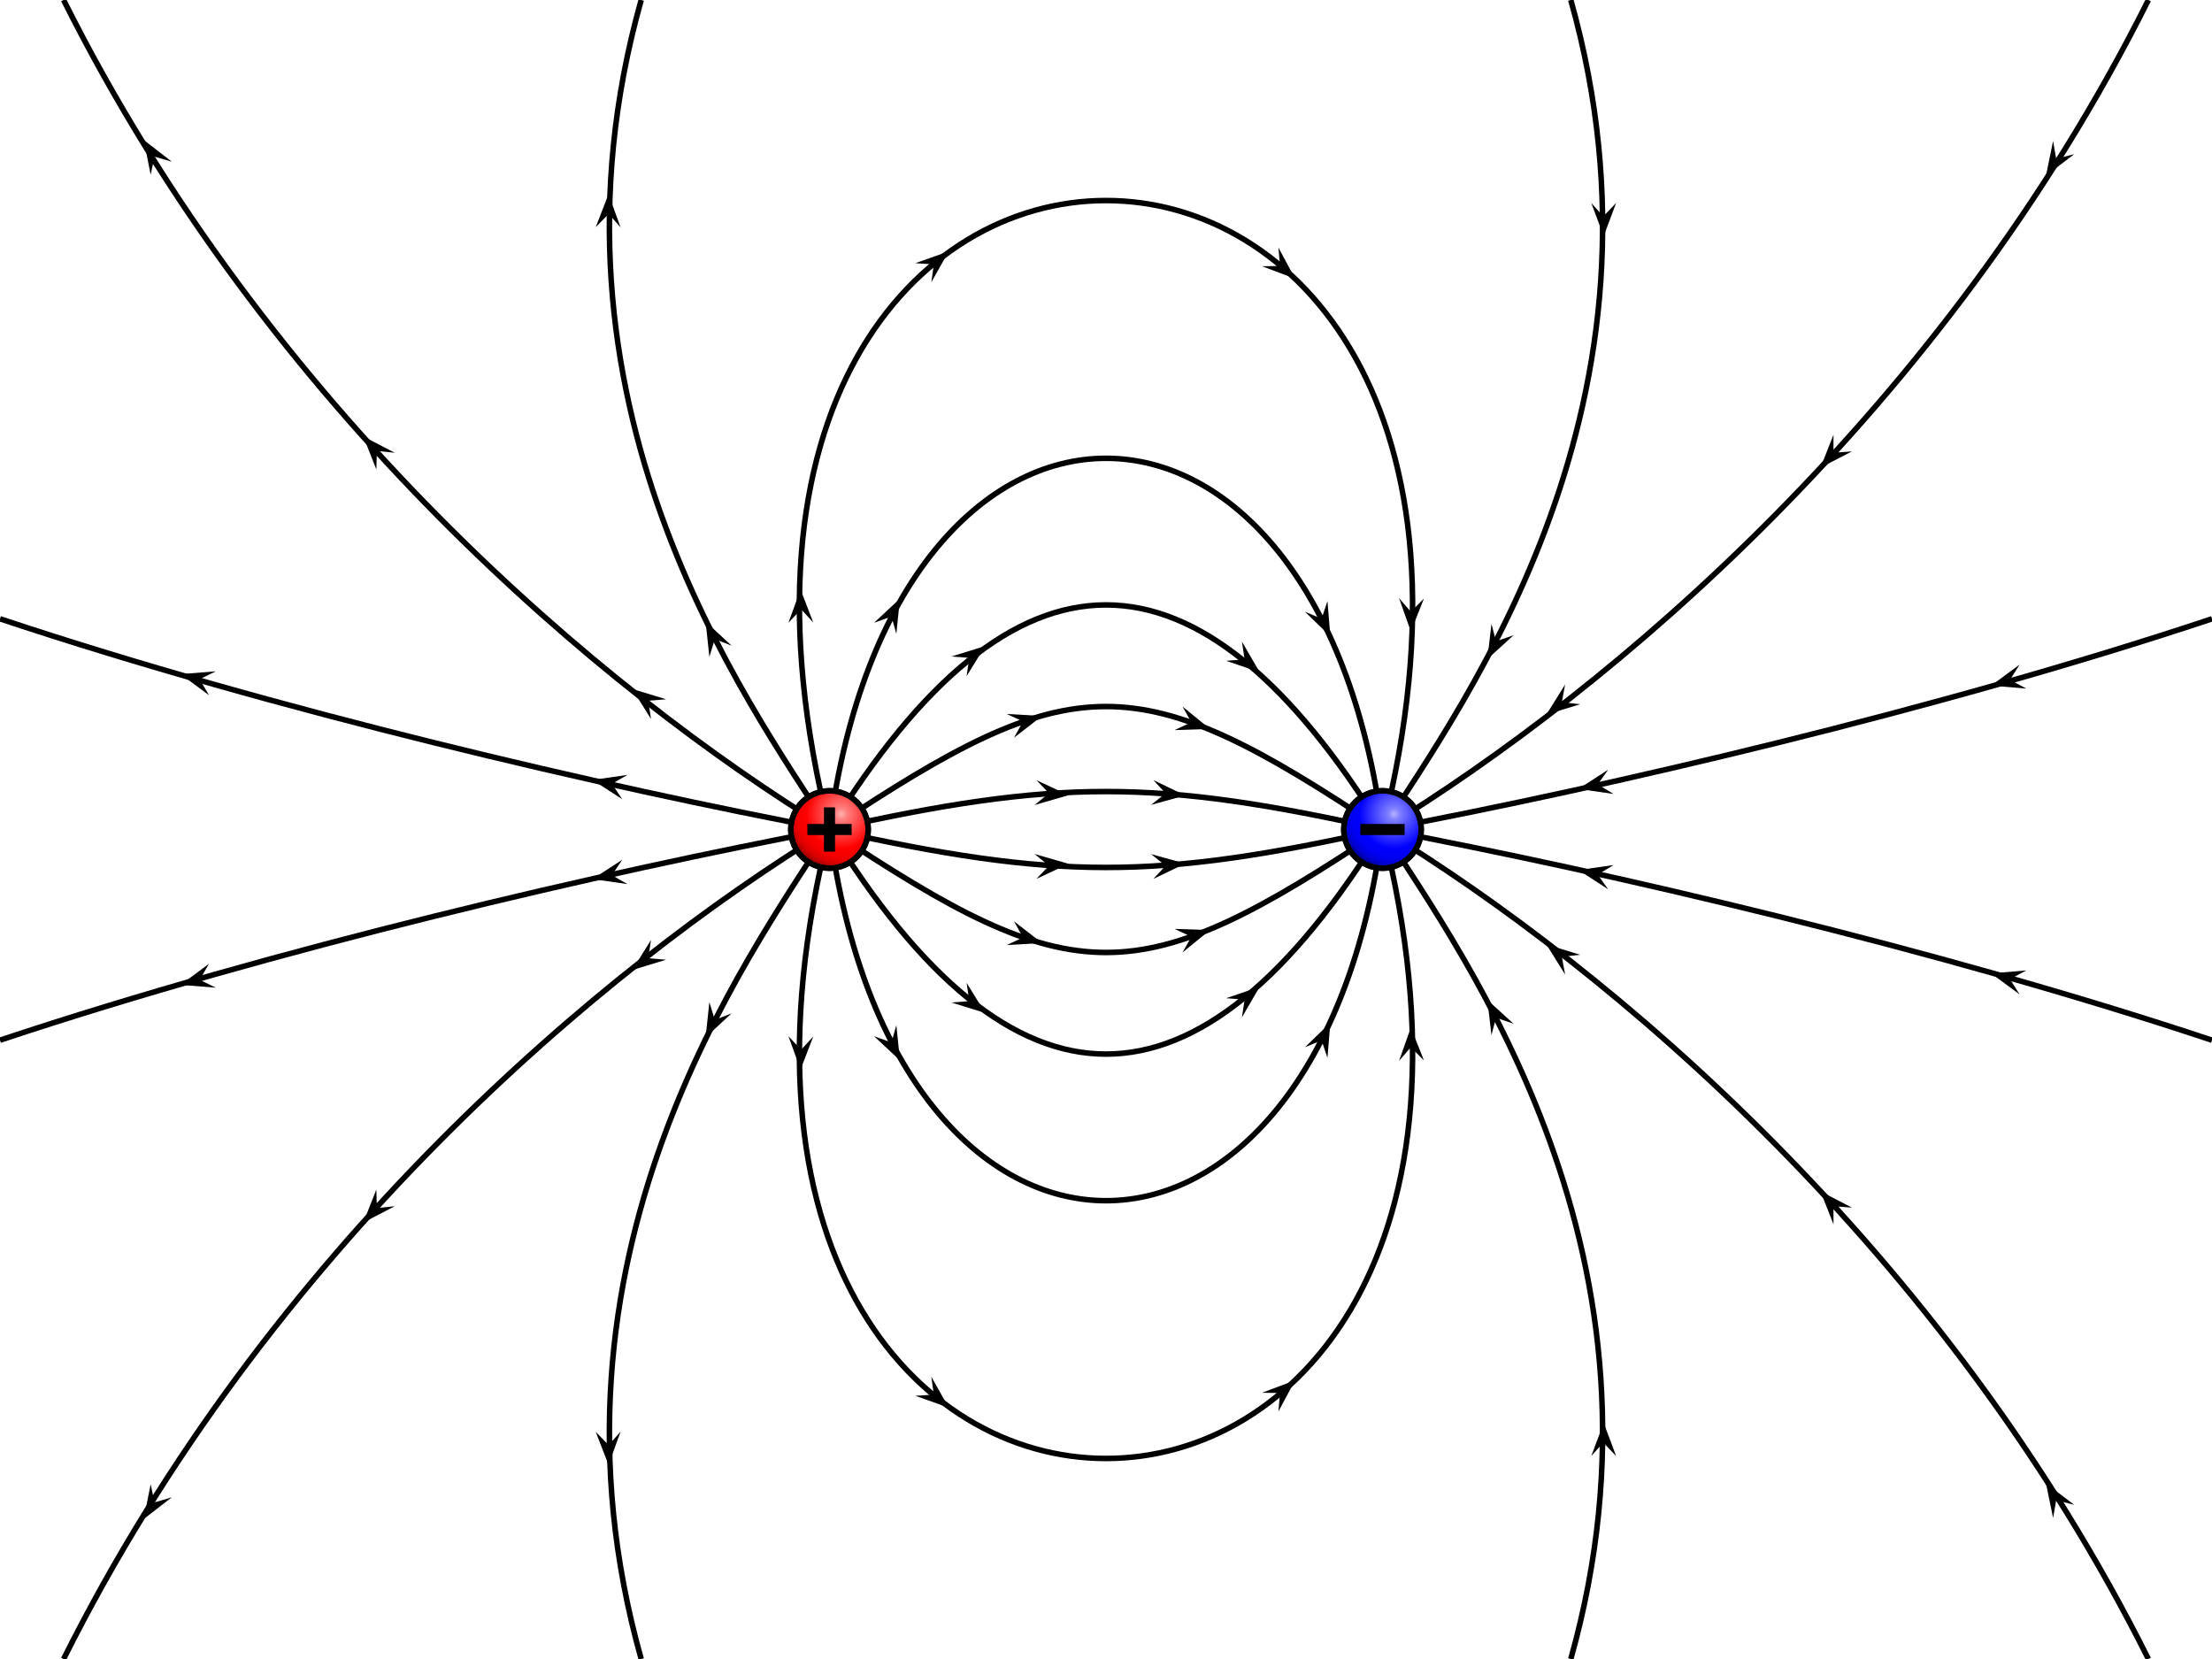
\includegraphics[width=8cm]{Bilder/field.png}
		\caption{Feldlinien von Punktladungen}
	\end{center}
\end{figure}



\subsubsection{Homologe Felder}
Zwischen zwei Kondensatorplatten herrscht ein homologes Feld. Zwischen ihnen verlaufen die feldlinien
direkt von + zu -. An den Randbereichen des Kondensators sind die Feldlinien gewölbt.

\begin{figure} [h]
	\begin{center}
		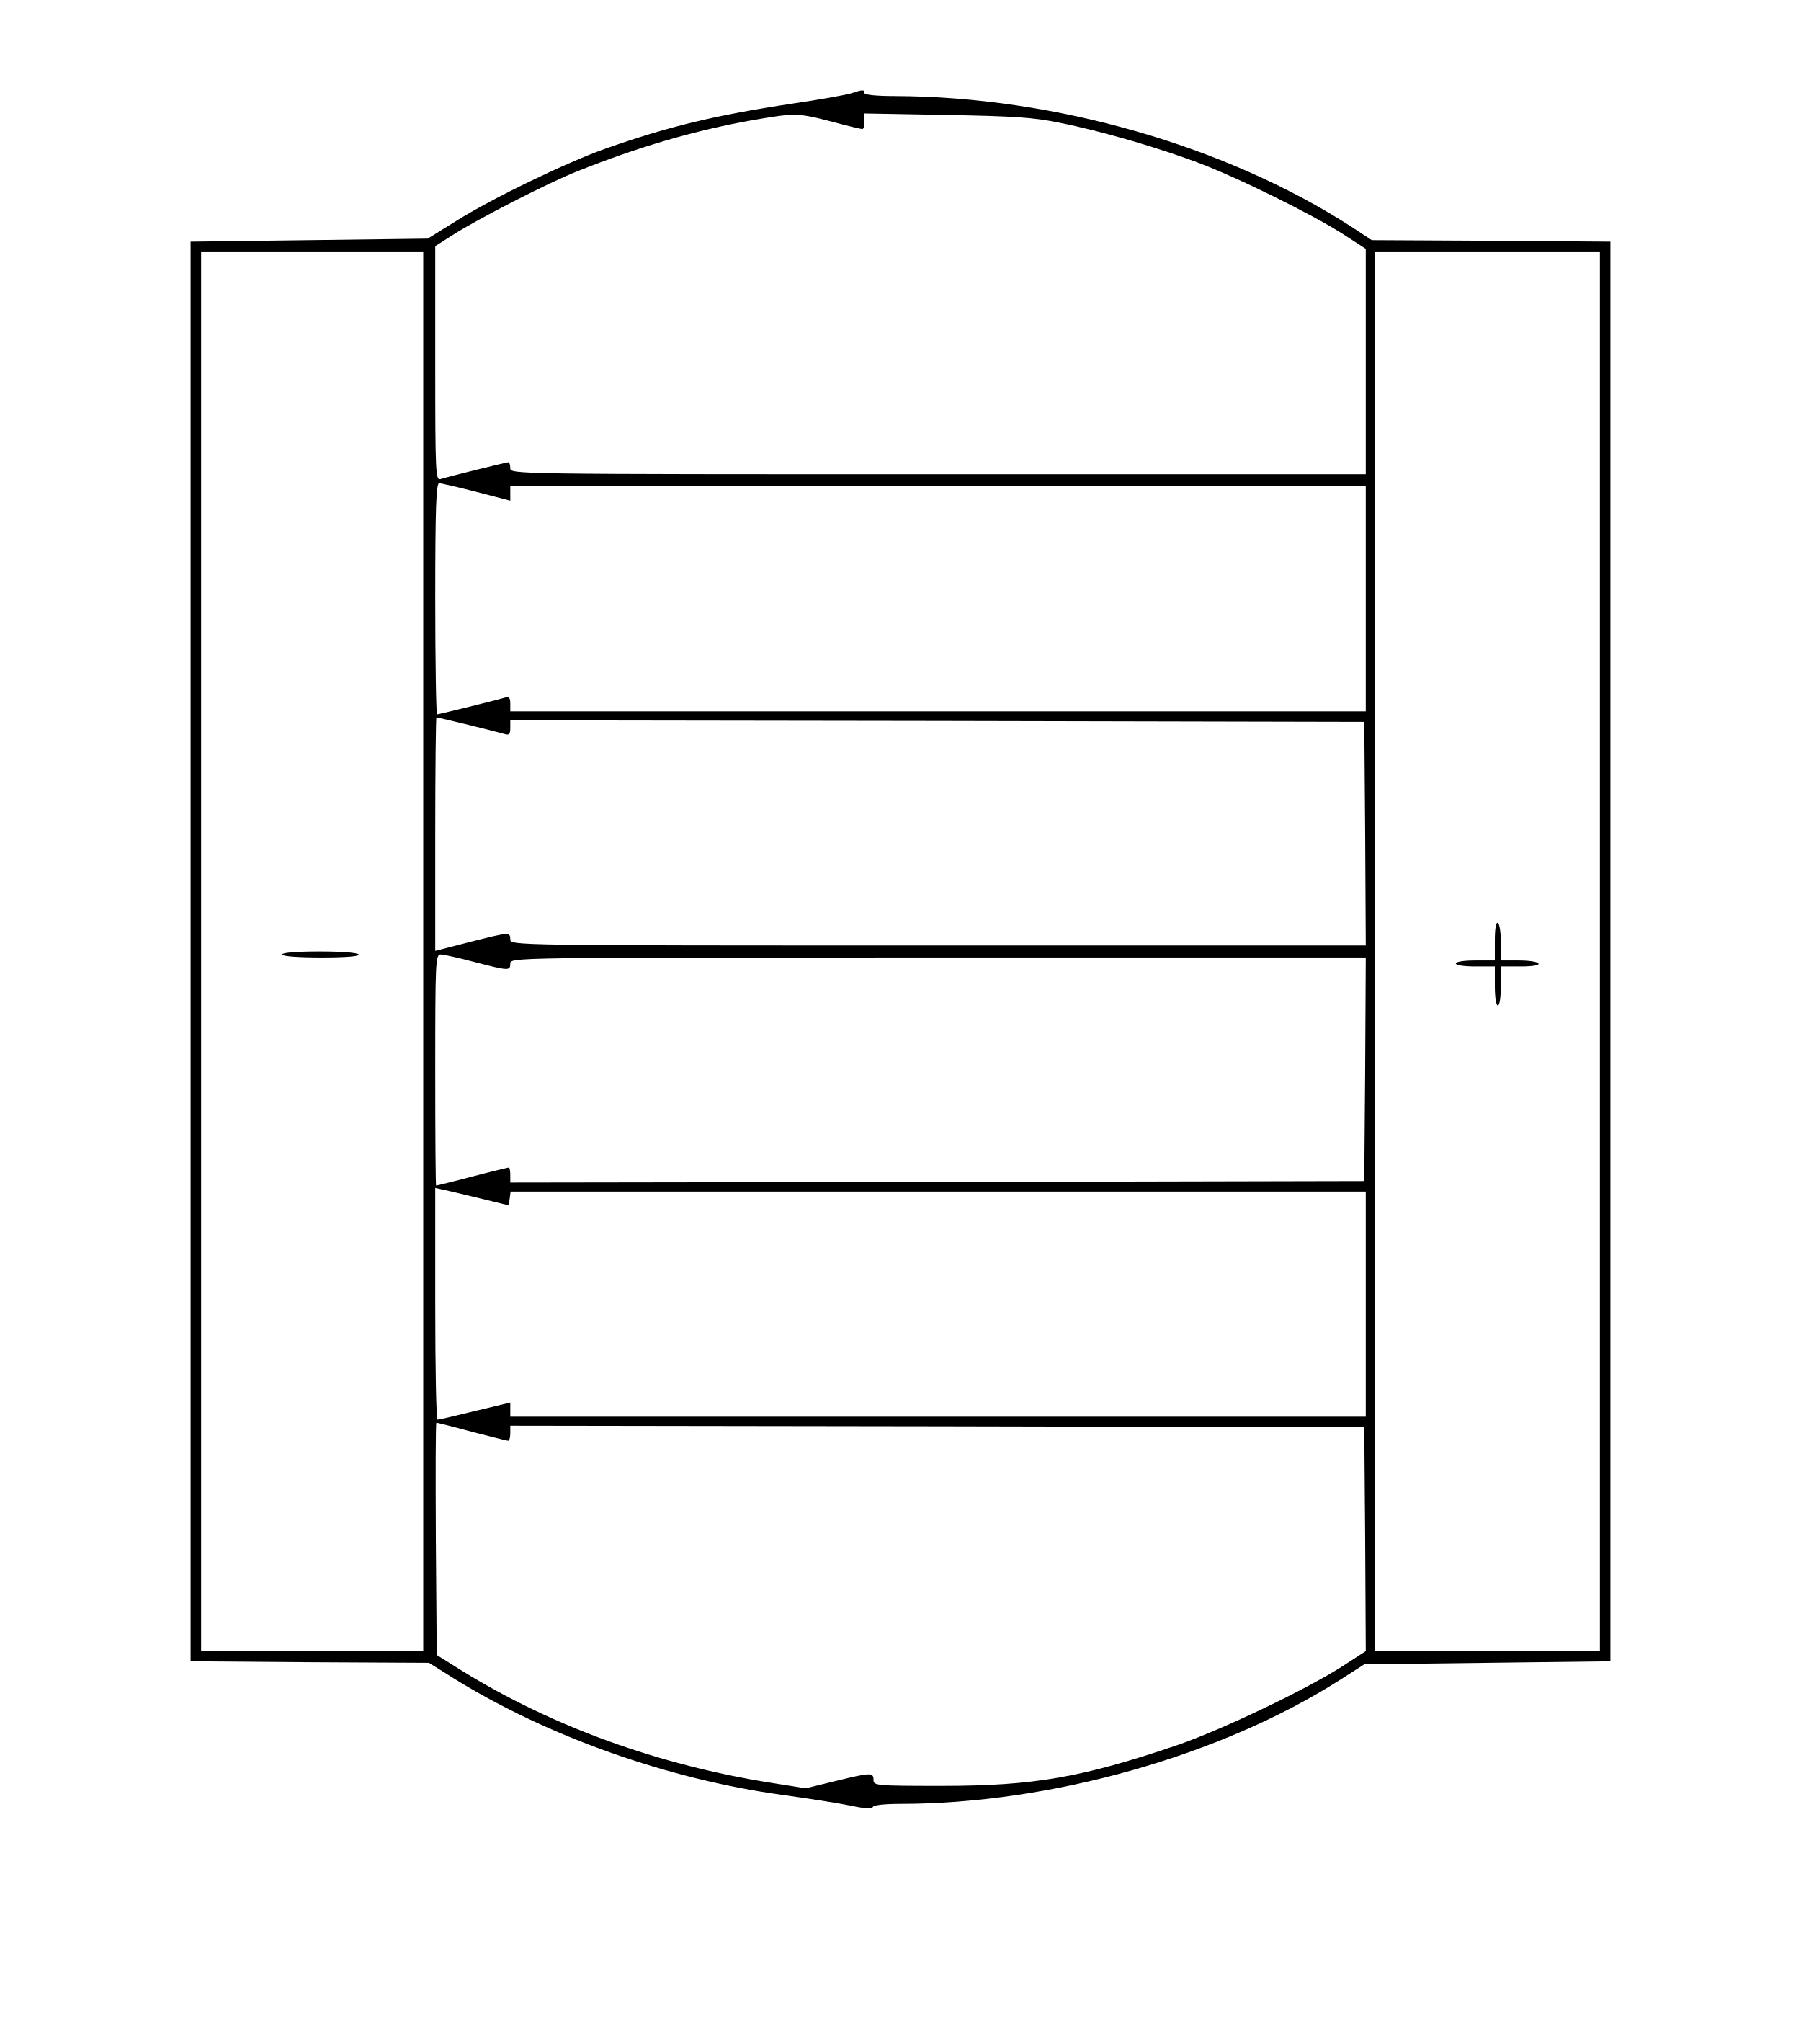
\includegraphics[width=8cm]{Bilder/homFeld.png}
		\caption{Feldlinien von homologen Feldern}
	\end{center}
\end{figure}



\subsection{Elektrische Feldstärke}
Die Elektrische Feldstärke ist proportional zur Kraft, die auf eine Probeladung wirkt und antiproportional
zur Ladung der Probeladung ($q$). Somit ergibt sich:

\Large$$\vec{E} = \dfrac{\vec{F}}{q}$$\normalsize\\




\subsubsection{Energie im homogenen elektrischen Feld}
Wenn sich eine Probeladung duch ein \textbf{homologes elektrisches Feld}, von einer Seite zur Anderen,
bewegt werden soll, wird eine Energie ($W$) benötigt. Diese berechnet sich durch:

\Large$$W = q \cdot \vec{E} \cdot d$$\normalsize

\begin{center}
	\vspace{0,4cm}oder
\end{center}

\Large$$U = \dfrac{W}{q} = \vec{E} \cdot d$$\normalsize\\

Daraus ergibt sich für die \textbf{elektrische Feldstärke im homogenen elektrischen Feld}:

\Large$$\vec{E} = \dfrac{U}{d}$$\normalsize\\



\subsection{Flächenladungsdichte}

Die Flächenladungsdichte ($\sigma$) ist definiert als Ladung pro Fläche. Somit gilt:$\sigma = \dfrac{Q}{A}$.\\
Mit dem proportionalitätsfaktor $\epsilon_0 (8,85\cdot10^{-12}\dfrac{As}{Vm}) \quad (\dfrac{As}{Vm} = \dfrac{C^2}{Nm^2})$ ergibt sich:\\
\Large$$\sigma = \epsilon_0 \cdot E$$\\ \normalsize

\textbf{Nur im Plattenkondensator} gilt außerdem:\\
\Large$$\sigma = \epsilon_0 \cdot \dfrac{U}{d}$$\\ \normalsize

Beim der Verwendung eines Dielektrikums gilt:\\
\Large$$\sigma \quad=\quad \epsilon_0 \cdot \epsilon_r \cdot \dfrac{U}{d} \quad=\quad \epsilon_0 \cdot \epsilon_r \cdot E$$\\ \normalsize


\subsection{Das Coulombsche Gesetz}

Zwei geladene Körper üben gegenseitig eine Kraft auf einander auf. Diese Kraft ist proportional zu beiden Ladungen
und antiproportional zum Quadrat ihres Abstands. Die Art der Ladung (positiv/negativ) spiegelt sich im Vorzeichen
der Ladungen wieder. Diese Kraft lässt sich wie folgt brechnen:\\

\Large$$F = \dfrac{1}{4\pi \epsilon_0} \cdot \dfrac{q_1 \cdot q_2}{r^2}$$\\ \normalsize




\section{Kondensatoren}
\subsection{Kapazität}

Die Kapazität ($C$) eines Kondensators ist proportional zur Ladung ($Q$) und antiproportional zur Spannung ($U$).
Somit ergibt sich für $C$:
\Large$$C = \dfrac{Q}{U}$$\\ \normalsize

Häufig wird zur Vergrößerung der Kapazität ein Isolator zwischen den Kondensatorplatten verbaut. Ein solcher Isolator
heißt Dielektrikum. Dessen Einfluss wird durch die \textbf{relative Permittivität ($\epsilon_r$)} beschrieben. Ein Vakuum besitz eine
relative Permittivität von $1$. Luft von $\approx 1$. Somit ergibt sich für die Kapazität eines Kondensators mit
Dielektrikum:\\
\Large$$C = \epsilon_0 \cdot \epsilon_r \cdot \dfrac{A}{d}$$\\ \normalsize



\subsection{Bewegung von Ladungsträgern im elektrischen Feldern}
\subsubsection{Parallel zur Feldlinie}

Wenn sich ein Ladungsträger parallel zu den Feldlinien bewegt, erfährt er eine Kraft ($F$) von $F = q \cdot E$.
Bei einer Bewegung über den gesamten Abstand der Kondensatorplatten gilt für die erhaltene Energie:
$W_a = F \cdot d = q \cdot E \cdot d = q \cdot U$\\
Da $W_{el} = W_(kin)$ gilt, ergibt sich für die Geschwindigkeit ($v$) nach Durchlauf des elektrischen
Feldes:\\
\begin{align*}
	\small \frac{1}{2}m \cdot v^2 &= q \cdot U\\
	 &\Updownarrow\\
	\Large v &= \sqrt{\dfrac{2qU}{m}}\\ \normalsize
\end{align*}



\subsubsection{Quer zur Feldlinie}

Nehmen wir an ein Ladungsträger passiert, wie in einer Braun'schen Röhre ein Elektron, ein Elektrischen Feld
quer zur Feldrichtung. Dann bewegt sich der Ladungsträger in x-Richtung mit konstanter Geschwindigkeit
($v_x = v_0 = \text{konstant}$). In y-Richtung wird die Ladung in Richtung des Pols mit entgegengesetzter Ladung
beschleunigt. Die y-Koordinate in Abhängigkeit zu x ist demnach:\\ $$y(x) = \dfrac{q \cdot U_y}{2 \cdot m \cdot d \cdot v_x ^2} \cdot x^2$$\\

Interessanter, z.B. auch für die bereits erwähnten Braun'schen Röhren, ist allerdings die Ablenkung des Ladungsträgers
nach Durchlauf der Gesamtlänge $l$:

\Large$$Y_1 = \dfrac{q \cdot U_y \cdot l^2}{2 \cdot m \cdot d \cdot v_x ^2}$$\\ \normalsize



\subsection{Energie im Kondensator}

Für die Energie im Kondensator gilt:\\

$$W = \frac{1}{2} \cdot Q \cdot U$$\\

Und da $Q = C \cdot U$ gilt, ergibt sich:

\Large$$W = \frac{1}{2} \cdot C \cdot U^2$$\\ \normalsize



\end{document}